\section{Fundamentação Teórica}
\label{sec:fundamentacao}

Nesta seção, apresentaremos o conceito de software livre e os motivos para
termos adotado ideologia no contexto deste artigo. Além disso, apresentaremos
a arquitetura e as principais características do Noosfero e do
\textit{framework} através do qual este foi desenvolvido, o
\textit{Ruby on Rails}.

%-----------------------------------------------------------------------------%
\subsection{Software Livre}

O princípio básico do ecossistema do software livre é promover a liberdade
do usuário, sem discriminar quem tem permissão para usar um software e seus
limites de uso, baseado na colaboração e num processo de desenvolvimento
aberto. Software livre é aquele que permite aos usuários usá-lo, estudá-lo,
modificá-lo e redistribui-lo, em geral, sem restrições para tal e prevenindo
que não sejam impostas restrições aos futuros usuários \cite{meirelles2013}.
Entendemos que este modelo de desenvolvimento de distribuição de software
seja o ideal em um estudo de caso envolvendo uma universidade, uma vez que
entendemos ser o papel da universidade não só promover a construção de
conhecimento, mas também a disseminação deste conhecimento para a sociedade,
e a utilização do software livre permite isso por causa dos quatro direitos
que este fornece%
\footnote{Extraído de \url{http://www.gnu.org/} em Julho de 2014}:

\begin{itemize}
  \item A liberdade de utilizar o software, para qualquer propósito;
  \item A liberdade de estudar como o software funciona e adaptá-lo para suas necessidades;
  \item A liberdade de redistribuir cópias para seus vizinhos;
  \item A liberdade de aprimorar o software, e redistribuir seus aprimoramentos para o público,
  de forma a beneficiar toda a comunidade;
\end{itemize}

%-----------------------------------------------------------------------------%
\subsection{Noosfero}

Noosfero é uma plataforma web livre para criação de redes sociais,
desenvolvida pela Cooperativa de Tecnologias Livres - Colivre, em 2007, sob
licença AGPLv.3, com a proposta de permitir aos usuários criarem sua própria
rede social personalizada, livre e autônoma.

O Noosfero foi desenvolvido na linguagem de programação Ruby%
\footnote{\url{http://www.ruby-lang.org/en/}},
versão 1.8.7, e utiliza o \textit{framework} Model-View-Controller (MVC) para
aplicações web Ruby on Rails%
\footnote{\url{http://rubyonrails.org/}}, versão 2.3.5.
%
A escolha destas tecnologias, por parte dos criadores do Noosfero, que também
trabalhamos juntos no contexto deste trabalho,
foi baseada no fato de que o Ruby possui uma sintaxe
simples, elegante e de fácil leitura, o que aumenta a manutenibilidade do sistema,
uma característica importante num projeto de software livre que visa atrair
desenvolvedores externos~\cite{meirelles2013}.
%
Outras características importantes que influenciaram essa escolha são a alta
capacidade produtiva que o \textit{framework} possui por priorizar conceitos como
\textit{convention over configuration} (convenção antes de configuração)
e DRY\footnote{Uma forma de apologia ao reuso de código}
(\textit{Don't Repeat Yourself} - Não Repita a Si Mesmo), bem como, o alinhamento
entre a comunidade do Ruby on Rails com metodologias ágeis de
desenvolvimento de software, que são evidenciadas em uma série de ferramentas que
viabilizam o uso de práticas como TDD\footnote{Desenvolvimento orientado a testes}
e BDD\footnote{Design orientado a comportamento}, práticas adotadas no
desenvolvimento do Noosfero, e neste trabalho.

Além disso, a arquitetura do Noosfero foi pensada para permitir que este seja facilmente
expansível, de forma que funcionalidades que não sejam comuns ao conceito de
redes sociais sejam desenvolvidas como \textit{plugins}, assim diminuindo
o acoplamento e aumentando a coesão dos diversos módulos do sistema.
%
Uma das grandes vantagens em se criar uma aplicação com arquitetura extensível
é a possibilidade de criar \textit{plugins} sem precisar modificar o código
fonte do núcleo da ferramenta, além de permitir o isolamento de \textit{bugs}
mais facilmente.

Essa abordagem arquitetural é muito benéfica para a diversidade de contextos
em que o Noosfero pode ser utilizado. Diversidade essa que pode ser evidenciada
quando se observa a existência de uma rede como o Cirandas%
\footnote{\url{https://cirandas.net/}},
uma rede social com o propósito de promover economia solidária através
da troca e venda de produtos e serviços, e o
Stoa, um ambiente virtual para a disseminação de conhecimento em âmbito
acadêmico de forma colaborativa, ambos desenvolvidos utilizando o Noosfero.
%
Dessa forma, os dois ambientes são instâncias do Noosfero que utilizam o seu
núcleo comum, mas diferem no uso de \textit{plugins} com funcionalidades
próprias às suas necessidades específicas.

\begin{figure}[htpb]
    \begin{center}
      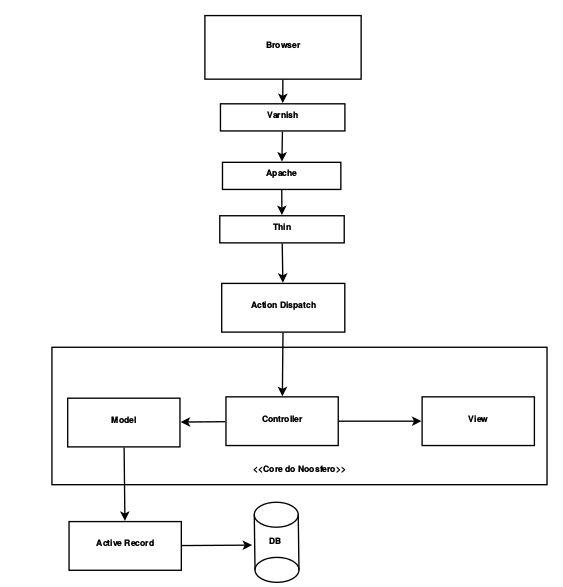
\includegraphics[width=.37\textwidth]{images/noosfero-architecture.png}
    \end{center}
    \caption{Visão arquitetural do Noosfero.}
    \label{noosfero-arch}
\end{figure}

A Figura \ref{noosfero-arch} apresenta uma visão arquitetural de alto nível
do núcleo do Noosfero. Vale a pena ressaltarmos alguns componentes desta arquitetura:

\begin{itemize}
    \item \textbf{Varnish:} acelerador de aplicações web também conhecido
    como cache de proxy reverso HTTP. É utilizado quando for necessário
    acessar conteúdo estático, imagens, \textit{scripts} e folhas de estilos.

    \item \textbf{Apache:} \textit{web-server} utilizado como servidor de
    \textit{proxy} reverso. Sua função é encaminhar as requisições que
    chegam para uma das instâncias do Thin.

    \item \textbf{Thin:} \textit{app-server} utilizado para processar as
    requisições de entrada e saída e encaminhá-las para o Noosfero para que
    ele possa executá-las. Pode ser configurado para utilizar mais de um
    processo para realizar balanceamento de carga. É recomendável o uso de
    dois processos do \textit{Thin} por núcleo de processador do servidor
    hospedeiro.

    \item \textbf{ActionDispatch:} funciona como roteador. Sua função é
    mapear as requisições que chegam a suas respectivas \textit{controllers}.

    \item \textbf{Controller:} controla o fluxo da aplicação. Realiza a
    ligação entre as entidades de \textit{model} e de \textit{view} através
    de chamadas de métodos.

    \item \textbf{Model:} representa as entidades do domínio da aplicação.
    A lógica da aplicação é implementado nas classes de \textit{model}.

    \item \textbf{View:} responsável pela visualização das páginas, isto é,
    as saídas em HTML da aplicação.

    \item \textbf{Active Record:} realiza o mapeamento entre os objetos de
    \textit{model} e o modelo relacional utilizado no banco de dados da
    aplicação.

\end{itemize}

